\chapter{Applications of Gomory-Hu Tree}
    After going through multiple research papers I observed that almost all, if not all applications of Static and Dynamic Gomory-Hu trees are on various Clustering Algorithms and Connectivity.

    \vspace{5mm}
    \noindent \textbf{Graph Clustering} problems aims at decomposing a given graph along sparse cuts into somewhat dense subgraphs called \textit{clusters}. It focuses on \textit{intra-cluster density} and \textit{inter-cluster sparsity}. Further clustering problems are used to get good heuristics in NP-hard problems that rely in finding good clusters.

    \begin{figure}[!htb]
        \centering
        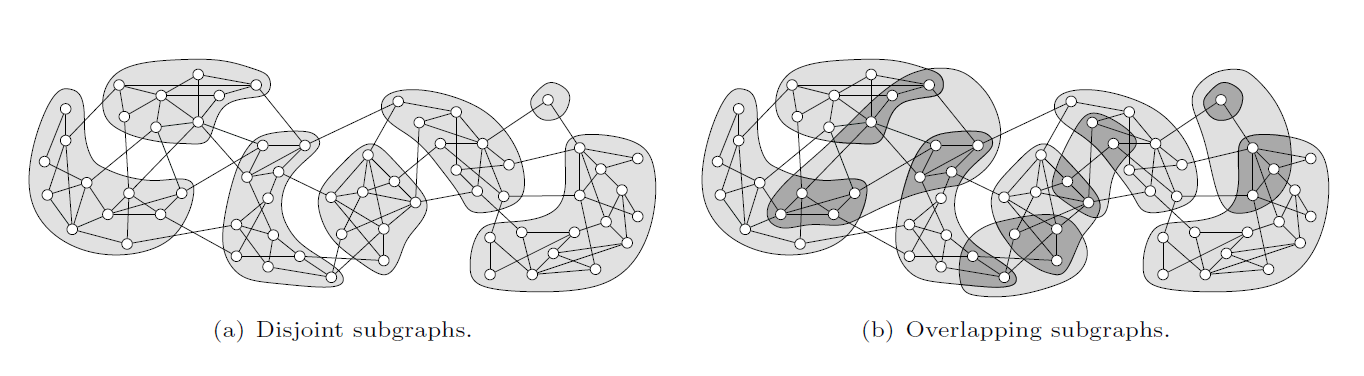
\includegraphics[width=1\linewidth]{figures/cluster.png}
        \caption{Decomposition of a graph into subgraphs}
        \label{cluster}
    \end{figure}
    \vspace{3mm}

    \noindent Some of the popular quality measure to measure clustering in a graph are - 
    
    \vspace{5mm}
    \noindent{\bf 1. Modularity} of clustering in an undirected unweighted graph is based on the total edge cost in $G$ that is covered by clusters with values ranging from -0.5 to 1, with 1 being the best value. Modularity $\mathcal{M}$ of a clustering $\Omega$ is defined as - 
    $$\mathcal{M}(\Omega) = \sum_{C\in \Omega}c(E_C)/c(E) - \sum_{C\in \Omega}(\sum_{v\in C} deg(v))^2/4c(E)$$ 

    \vspace{5mm}
    \noindent{\bf 2. Expansion} is a quality measure of cuts in weighted graphs. Higher the expansion the better. Expansion $\psi(U,C\backslash U)$ of a clustering $(U,C\backslash U)$ is defined as - 
    $$\psi(U,C\backslash U) = \frac{c(U,C\backslash U)}{min(|U|,|C\backslash U|)}$$ 

    \vspace{5mm}
    \noindent{\bf 3. Conductance} is a quality measure of cuts in weighted graphs. Lower the conductance the better. Condutance $\phi(U,C\backslash U)$ of a clustering $(U,C\backslash U)$ is defined as - 
    $$\phi(U,C\backslash U) = \frac{c(U,C\backslash U)}{min(deg(U),deg(C\backslash U)}$$ 

    \noindent Among the Cut-based Clustering techniques commonly used are - 
    
    \vspace{2mm}
    \noindent{\bf 1. Static Hierarchies of Cut Clustering} - Aim is to compute and organize all relevant minimum cuts of a graph into a nested hierarchical structure to form a hierarchy of clusters, so that the global cut structure of the graph can be further examined/analyzed. One algorithm for this was presented by Flake et al. that exploits the propoerties of minimum separating cut together with an input parameter $\alpha$ to find hierarchial clustering $C$.

    \vspace{5mm}
    \noindent{\bf 2. Maximum Source-Community Clustering} - identifies \textit{communities} in a graph by repeatedly finding min-Cuts that best separate a chosen vertex from the rest of the graph. It can be used for Community Detection, Hierarchial Clustering Tree, etc.

    \vspace{5mm}
    \noindent{\bf 3. Unrestricted Cut-Clustering Algorithm} Similar to previous one this also aims at finding communities in a graph but without any restrictions on the end vertices $s-t$.

    \vspace{5mm}
    \noindent{\bf 4. Fully Dynamic Hierarchies of Unrestricted Cut-Clustering Algorithm} Instead of a Static unrestricted Cut-Clustering, this one accommodates for mobility in the clusters do dynamically update and detect or erase newer clusters. Similar to Dynamic Gomory-Hu trees this one also supports concrete changes on a concrete edge and finding changes at each step.

    \vspace{5mm}
    Some of the major/significant Applications of Gomory-Hu Tree as given in various research papers are:
    \begin{enumerate}
        \item {
            \textbf{Image Segmentation [WL93]:} Given an input image our goal is to partition the image into various parts, such that each part has some meaningful interpretation. While there are many do Image Segmentation including usage of Convolutional Netural Networks, here we are going to Segment the image by converting it into a graph and partition based on Cut-values between nodes. \\ 
            More about this is discussed in the next chapter.
        }

        \item {
            \textbf{Identifying protein complexes in Protein-Protein Interaction(PPI) [JM20]:} Y2H (Yeast two-hybrind) PPI networks comprise proteins (nodes) and interactions of the type Y2H (edges). In the view of graph theory, a PPI network is an undirected and unweighted network. The intuition being - A protein complex should have strong internal connectivity and relatively weak external connectivity. \\
            Additionally, with the use of Sensitivity and Parametric analysis of Dynamic Gomory-Hu Trees one can efficiently filter out False Postives and Negatives. 
        }

        \item{
            \textbf{Optimal Service Component Distribution across Multiple Clouds [DA18]:} Service Request in a Multi-Cloud Model can be expressed as a complex topology with nodes and links constraints. The goal is to decompose the request into sub-request and try to minimize the number of partitions that can be mapped to at least one cloud provider meeting the user requirements. This decomposition step is done using Gomory-Hu Tree to cluster/parition into multiple clouds.
        }

        \item{
            \textbf{Finding All k-Edge-Connected Components [Tia15]:} Given a graph $G = (V, E)$, the problem is to partition the vertex set $V$ into ${V_1,V_2,. . ., V_h}$, where each $V_i$ is maximized, such that for any two vertices $x$ and $y$ in $V_i$, there are $k$ edge-disjoint paths connecting them.
        }

        \item{
            \textbf{Collaborative Uncapacitated Arc Routing Problem:} The goal is to maximize profit in a network with multiple carriers and each of them Collaboratively/Collectively work to optimize a given function (such as travel cost). Assuming that the nodes have no binding capacity constraints.
        }

        \item{
            \textbf{Graph b-coloring for Data Clustering [HH08]:} \textit{b-colouring} is a special case of \textit{proper b-colouring} where there exists a special vertex \textit{u (dominating vertex/b-vertex)} which is adjacent to at least one other vertex in every other colour class. This is used in Clustering since the \textit{b-vertex} can be used as a boundary object between two different classes and helps to distinguish clusters clearly.
        }

        \item{
            \textbf{Joint Interference and User Association Optimization in Cellular Wireless Networks [Cr13]:} In wireless networks users must connect to base stations. In modern network the best stations it not necessarily the nearest one. Here, we attempt to decompose the problem into smaller subproblems and then use min-cut to find bottlenecks and boundaries in the network.
        }
    \end{enumerate}